Para poder utilizar las técnicas de blindaje contra ondas de superficie utilizando metamateriales, como las descriptas en el informe, es necesario que el ancho de la banda prohibida de la estructura EBG resulte mayor al ancho de banda de la antena. Es debido al alto valor del factor Q (y por tanto, bajo ancho de banda) de las antenas \textit{microstrip} rectangulares el motivo por el que el uso de estructuras EBG es factible.
La caracterización del comportamiento de las estructuras de banda prohibida electromagnética ubicadas entre antenas \textit{microstrip} para frecuencias más allá de la de resonancia escapa del objetivo de este trabajo. Sin embargo, el tema se trató repetidas veces durante el desarrollo del trabajo, especialmente debido a que se debió considerar la viabilidad de realizar mediciones de caracterización del EBG para realizar comparaciones con las simulaciones obtenidas. Este apéndice pretende introducir conceptualmente el tema.

Existen numerosas técnicas que permiten aumentar el ancho de banda de las estructuras radiantes de tecnología \textit{microstrip}. Como se explicó antes, una técnica común consiste en aumentar al ancho del sustrato, o cambiarlo por otro de constante dieléctrica menor. Debido a que la modificación de cualquiera de los dos parámetros condicionaría sustancialmente el comportamiento de las ondas de superficie generadas sobre el sustrato, se decidió que resultaba importante independizarlos del análisis.

En otros casos, se ha propuesto la modificación de la geometría del elemento radiante, descartando el tradicional parche rectangular por figuras con formas de U o de E, o por formas geométricas con aperturas radiantes embebidas \cite{Yang:EBGAntennas}. Para las mediciones de este trabajo se consideró, y finalmente se descartó, el uso de antenas \textit{microstrip} de tipo moño (\textit{bow-tie}), que presentan una transición geométrica suave, intuitivamente apta para las necesidades presentadas. Entre las dificultades que ofrece, está su principio de funcionamiento, comparable al de un dipolo, y requiriendo, por tanto, una alimentación en modo diferencial, lo que obligaría a realizar un diseño de un balún \textit{microstrip}, lejano a las pretensiones del trabajo.

Otra técnica común consiste en diseñar conjuntos de elementos que resuenan a distintas y frecuencias, acoplados capacitivamente, denominados estructuras multi-resonantes. Si las distintas frecuencias de resonancia están lo suficientemente cerca unas de otras, se logra un efecto de continuidad, aumentando notoriamente el ancho de banda. En muchos casos, y debido a los costos cada vez más despreciables de la fabricación de circuitos multicapa, los elementos resonantes se ubican apilados, generando un acoplamiento capacitivo máximo entre ellos. Para el caso de las pruebas que se requieren hacer para validar y caracterizar el comportamiento de las estructuras EBG, elementos radiantes coplanares con el parche activo resonante resultan suficientes.

La estructura propuesta consiste en un parche rectangular, ubicado sobre un sustrato de FR4, de comportamiento resonante en una frecuencia aproximada de 2.4 GHz, y ubicado entre dos rectángulos \textit{microstrip} pasivos iguales, de un largo establecido de forma que la frecuencia de resonancia de los mismos resulte ligeramente diferente a la del parche activo. La distancia entre estos elementos de carga y la antena original debe ser tal que el acoplamiento sea notorio, requisito que presenta complejidades \cite{Kumar:radiating} debido a que los parches deben estar ubicados frente a los bordes no radiantes de la antena para evitar reducir el espacio utilizado por la estructura EBG con la que compartirán sustrato. En la figura \ref{fig:antena-propuesta-con-ebg} se puede observar el arreglo final de elementos. Se debe destacar que la elección de que ambos parches posean las mismas propiedades geométricas se debe a la búsqueda de la máxima simetría par para simplificar el análisis de la estructura, aún cuando esta elección merme la flexibilidad del diseño de banda ancha.

\begin{figure}[h]
	\centering
	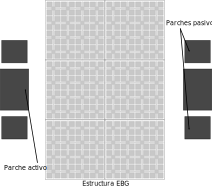
\includegraphics[width=0.9\textwidth]{Aplicacion/estructura-antenas-ebg.pdf}
	\caption{Estructura propuesta para la caracterización del efecto de EBGs sobre antenas microstrip.}
	\label{fig:antena-propuesta-con-ebg}
\end{figure}


Los parches rectangulares, al igual que en el desarrollo del análisis de estructuras EBG, están acoplados al elemento activo mediante lo que puede modelarse como una red $\pi$ de capacitores (acoplamiento capacitivo) \cite{Kumar:Non-radiating}, similar a mostrada en la figura \ref{fig:acoplamiento-capacitivo-modelo}, donde los denominados \textit{pixeles} deben ser reemplazados por los parches propiamente dichos. En términos generales, los parámetros que modificarán la impedancia de entrada y que, por lo tanto, afectarán al ancho de banda, son la distancia entre el resonador activo y los pasivos ($g'$), la longitud de los parches acoplados ($l'$) y la posición del punto de alimentación \cite{Kumar:Non-radiating}.

La existencia de estos parches, que pueden considerarse como de carga, implican una modificación de la impedancia de entrada para distintas frecuencias.

Si los parches pasivos poseen dimensiones muy disímiles al parche activo central, las frecuencias de resonancia de los elementos estarán tan alejadas entre sí que es posible un análisis simplificado del comportamiento: A bajas frecuencias, los rectángulo pasivos no resuenan ni se acoplan visiblemente al parche activo. A medida que la frecuencia de trabajo aumenta, los mismos comienzan a acoplarse, adoptando un comportamiento capacitivo, al mismo tiempo que debido a que forman un paralelo con la carga impuesta por la resistencia de radiación, disminuyen el valor de la resistencia de entrada. Una vez que los parches resuenan, logrando que se presente la mínima resistencia de entrada, obtienen un comportamiento de carácter inductivo, hasta que nuevamente, a altas frecuencias, dejan de tener injerencia palpable sobre el valor de la impedancia de entrada. La variación de la distancia entre los parches da lugar a que estos efectos se vuelvan más o menos plausibles, en función del acoplamiento capacitivo \cite{Kumar:Non-radiating}.

Cuando los parches pasivos poseen geometrías similares a la del parche original, el problema resulta más complejo, debido a que no puede analizarse la resonancia de cada elemento por separado sin considerar la carga que los demás ejercen sobre él. Debido a que, a fin de aumentar el ancho de banda, todos los parches deberán tener geometrías similares, resulta necesario realizar simulaciones numéricas que permitan predecir el comportamiento.

Para observar el efecto del uso de parches \textit{microstrip} acoplados capacitivamente al parche activo principal para aumentar el ancho de banda del sistema radiante, se realizaron sucesivas simulaciones en el software de simulación CST Microwave Studio, realizando una optimización para obtener el mayor ancho de banda posible dentro del rango de interés. Los parches deben ser de un largo similar a la antena, aunque ligeramente diferente, para aumentar el ancho de banda. Por otro lado, se eligió que fueran simétricos, a fin de no aumentar la anisotropía del problema.

Resulta conveniente, en este caso, realizar simulaciones para comprender el efecto de la variación de distintos parámetros, en particular de la distancia entre el radiador activo y los parches, $g'$, el ancho $w'$ de los parches y su largo $l'$. Las primeras simulaciones, utilizando los valores obtenidos en el análisis de un parche único, demostraron que los parches de carga efectivamente cambian las frecuencia de resonancia. 

En la figura \ref{fig:unparche-concarga-sinebg-varAnchoLprima} se puede observar el comportamiento, para distintos valores de $l'$, con $w'$ y $g'$ fijos, habiendo elegido los valores del parche óptimos obtenidos antes (donde se consideró un parche sin carga). Se observa que para todos los valores de $l'$ probados, la frecuencia de resonancia del sistema, o la frecuencia para la que el parámetro $S_{11}$ es mínima, disminuye notablemente, debido al acoplamiento entre elementos y la aparición de modos de menor frecuencia. En todas las curvas se observan dos mínimos locales. Cuando las cargas tienen un largo $l'$ menor al de la antena \textit{microstrip}, como es el caso para 25 mm y 28.75 mm, existe un mínimo a una frecuencia superior a la buscada, que para el caso de 25 mm queda fuera de la gráfica. De la misma manera, cuando el largo de las cargas es mayor al del parche, se presenta un mínimo a una frecuencia inferior. Como se explicó antes, el caso óptimo se da cuando ambos mínimos coinciden o están lo suficientemente cerca en frecuencia para aumentar el ancho de banda del sistema radiante. Se observa, también, que el mínimo absoluto del parámetro $S_{11}$ adopta un valor menor, más deseable, para valores de $l'$ por debajo de $L$, mientras que se ubica en una posición más cercana a la frecuencia buscada para valores por encima de $L$. Esta última variación podría controlarse mediante la disminución del tamaño de la geometría completa.

En la figura \ref{fig:unparche-concarga-sinebg-varDistanciaCarga} se puede observar que una mayor distancia entre el parche \textit{microstrip} y las cargas da lugar a una frecuencia de resonancia menor. Sin embargo, el mínimo local cercano a 2.17 GHz generado por la presencia de los parches de carga no varía notoriamente con la distancia. Por otro lado, el valor que adopta el mínimo absoluto parece ser menor cuando la distancia es pequeña.

Finalmente, en la figura \ref{fig:unparche-concarga-sinebg-varAltoWprima} se muestra la variación del comportamiento en frecuencia del parámetro $S_{11}$ en función de la variación del ancho $w'$ de los parches carga. La frecuencia donde se ubica el mínimo absoluto es mayor cuando el parche carga es angosto, ya que limita la formación de modos indeseados.

\begin{figure}[H]
	\centering 
	\subfigure[Variación del largo $l'$.]{
		\label{fig:unparche-concarga-sinebg-varAnchoLprima}
		\includegraphics[width=0.47\textwidth]{Aplicacion/VariacionAnchoLprima-UnParcheConCarga.pdf}}
	\subfigure[Variación de la distancia entre la carga y el parche, $g'$.]{
		\label{fig:unparche-concarga-sinebg-varDistanciaCarga}
		\includegraphics[width=0.47\textwidth]{Aplicacion/VariacionDistanciagprimera-UnParcheConCarga.pdf}}
	\subfigure[Variación de valor de $w'$.]{
		\label{fig:unparche-concarga-sinebg-varAltoWprima}
		\includegraphics[width=0.50\textwidth]{Aplicacion/VariacionAltowprima-UnParcheConCarga.pdf}}
	\caption{Variación del parámetro $S_{11}$ del puerto en función de distintos parámetros del parche único, y antena optimizada final.}
	\label{fig:simulaciones-microstrip-1parchecargado}
\end{figure}

% Analizar por qué pasan cosas raras.
% Poner foto del diseño del único parche cargado final.
